%!TEX root = ./../thesis.tex

\chapter{Consistency Management}
\label{c:consistency_mgmt}
Consistency management in the context of distributed machine learning describes the process of ensuring an algorithm is parallelized most efficiently without loosing its correctness.
Iterative-convergent algorithms are mostly sequential in nature and parallelization is commonly achieved by exploiting their inherent stochastic properties.
Staying with the example of the previous section, as shown in Figure \ref{fig:ica_control_flow}, unit $\Omega_2$ of training step (C) is parallelized with a dop of $K = 2$ by partitioning the input data $D$ and replicating the model $w$ across all parallel units $\{\Omega_{2j}\}_{j=0}^K$.
Proper consistency management targets two domains of the algorithm execution process.
First, as discussed in Section \ref{ss:synchronization}, the control-flow must be synchronized properly according to the transformation applied during the execution of a unit $\Omega_i$ and its replicas $\{\Omega_{ij}\}_{j=0}^K$.
In the example, the loop in (B) and its containing units $\Omega_{2j}$ are defined as SSP in order to increase the data throughput on the input data $D$.
Ultimately this supposed to result in a better overall performance due to a lower dependency on other units.
Unfortunately, increasing the data throughput alone does not necessarily lead to a better overall performance, as each unit $\Omega_{2j}$ now works independently on a replica $w_j$ of the model without sharing the local progress.
As discussed in Section \ref{ss:consistency} this staleness of state has a negative effect on the algorithm throughput and can be mitigated by frequently exchanging the updates applied to a state, in this case $w$, between all units $\Omega_{2j}$.
Exchanging updates on the other hand has a negative effect on the data throughput as more computation time must be spent on network management.
Adaptive consistency management therefore is responsible for controlling the best trade-off between communication and computation, based on the requirements for synchronization and consistency at each step of the algorithm as well as continuous feedback about cluster metrics and algorithm progress.

\section{Adaptive Consistency Management}
Consistency management in general can be seen as a cooperative task between the driver and the machines involved in executing the workload defined by the algorithm definition.
Figure \ref{fig:adapt_consist_mgmt} depicts the architecture and connections between driver and machines, where the interpreter is responsible for instructing the machines according to the program flow and also taking care of managing units and states.
\begin{figure}[ht]
\centering
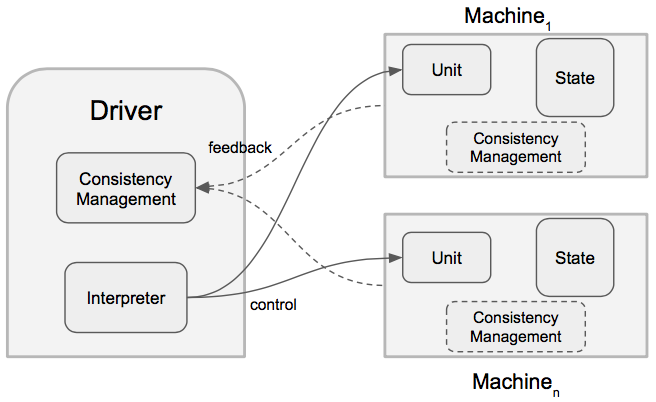
\includegraphics[width=0.7\textwidth]{img/adapt_consist_mgmt.png}
\caption{Adaptive Consistency Management Architecture}
\label{fig:adapt_consist_mgmt}
\end{figure}
The first part of the consistency management resides on the driver and is responsible for collecting feedback from the machines.
This is then used to exercise further control over the algorithm execution.
Feedback can be metrics about the machines, such as resource usage, network bandwidth consumption or algorithm specific properties such as the convergence rate.
Based on the collected feedback, the consistency management is able to provide instructions for the interpreter in order to influence the consistency on a unit level.
such as the synchronization between parallel instances of a unit in order to improve the algorithm throughput.
Furthermore, the second part of the consistency management resides on each machine.
This is necessary to gain control over the state level consistency as discussed in the previous section.
Consistency management on a state level becomes necessary when a unit is parallelized by creating replicas on multiple machines.
Parallelizing a unit results in replication or partitioning of the attached states and therefore
This part for example can be used to control the communication frequency of model or parameter updates based on the available network bandwidth or some network quota.
Also it is in general possible to control algorithm specific parameters such as the learning rate based on the progress of the other parallel units.
This generic architecture allows to cover a variety of different use-cases in consistency management.
While unit level consistency can be achieved solely by the interpreter via control-flow, state-level consistency requires more effort and coordination by the consistency management.
In algorithm steps where a unit is parallelized, state level consistency management depends mainly on the partitioning of the attached states as well as the access pattern.
\begin{figure}[ht]
\centering
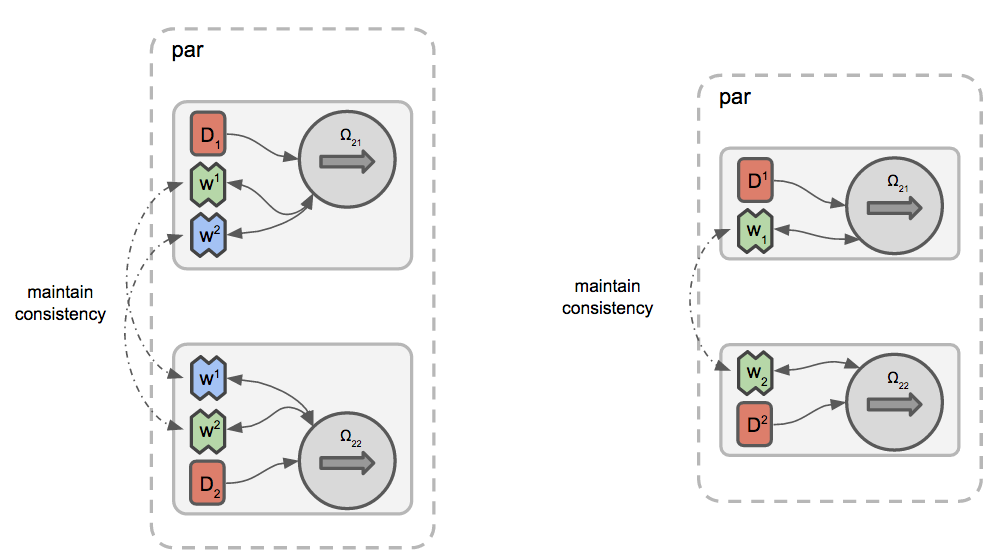
\includegraphics[width=0.9\textwidth]{img/par_repl_model.png}
\caption{Partitioned and Replicated State}
\label{fig:par_repl_model}
\end{figure}
As depicted in Figure \ref{fig:par_repl_model}, read-only states such as the input data $D$ are not subject to consistency management, whereas states that are altered by more than one unit in parallel must be kept consistent.
This stems from the fact that during the execution of a unit in parallel a non read-only state is in general subject to local and remote updates.
Depending on the partitioning the strategy to keep a state consistent varies slightly.
In case a state is partitioned across machines, there exists a main partition for each part of the state, containing the source of truth.
All units working in parallel on this part of the state, communicate the updates to the machine holding the main partition and also fetch the latest updates from this partition.
On the other hand, if a state is replicated there is no main partition holding the latest version of the state.
In this case each unit either has to broadcast all updates to all other parallel units or the units have to elect a unit that acts as the source of truth.
E.g. in case of the example depicted in Figure \ref{fig:ica_control_flow_dist}, unit $\Omega_{2i}$ updates its model $w_i$ locally based on some update procedure $\Delta$, according to (\ref{eqn:local_delta_upd}), but also receives the models $w_j, j \neq i$ of units $\Omega_{2j}, j \neq i$ as it is necessary to incorporate the progress of parallel instances in order to increase the algorithm throughput and mitigate slower convergence due to stale models.
The frequency at which the progress communication takes place is controlled by the consistency management based on the collected feedback.
As the second part of the consistency management must be present on each machine, the question arises which part on these machines is best suited to be responsible for controlling the consistency on a state level.

\section{State-centric vs. Computation-centric}
From an architectural perspective, two solutions can be considered for integrating the consistency management into each machine.
First, with state-centric consistency, as depicted in Figure \ref{fig:state_centric_consistency}, the consistency management is part of the state itself.
\begin{figure}[ht]
\centering
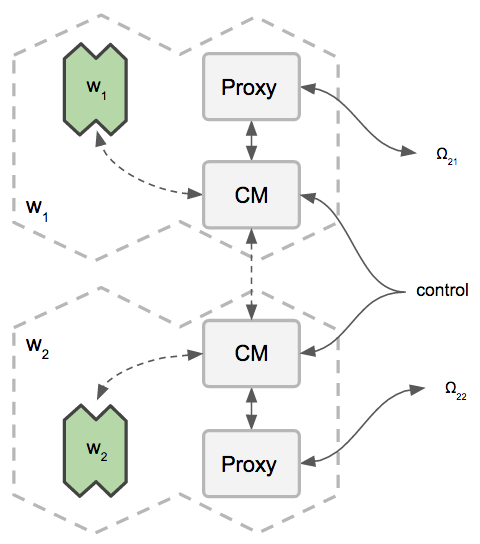
\includegraphics[width=0.5\textwidth]{img/state_centric_consist.png}
\caption{State-Centric Consistency Management}
\label{fig:state_centric_consistency}
\end{figure}
The consistency management and actual state are hidden behind a proxy, which mimics the interface of the state.
Each update is forwarded to the consistency management, which takes care of updating the local state as well as communicating updates to all other replicas or partitions depending on the partitioning.
The CM\footnote{Consistency Management} related parameters can be controlled by the driver.
This has the advantage that it offers a very convenient way to interact with a state because from a unit perspective a state behaves similar to a non-parallel version.
Furthermore, the design of a unit is considerably simplified as the computation is just a function that must be executed in parallel on multiple units and therefore very lightweight.
On the other hand, this approach requires a deep integration of consistency management logic into the state and therefore induces a tight coupling between logic and data.
This unnecessarily increases the dependency between data and framework and requires the developer to reimplement the logic in case the type of state changes.

Second, with computation-centric consistency, as can be seen in Figure \ref{fig:computation_centric_consistency}, the consistency management is part of the unit.
\begin{figure}[ht]
\centering
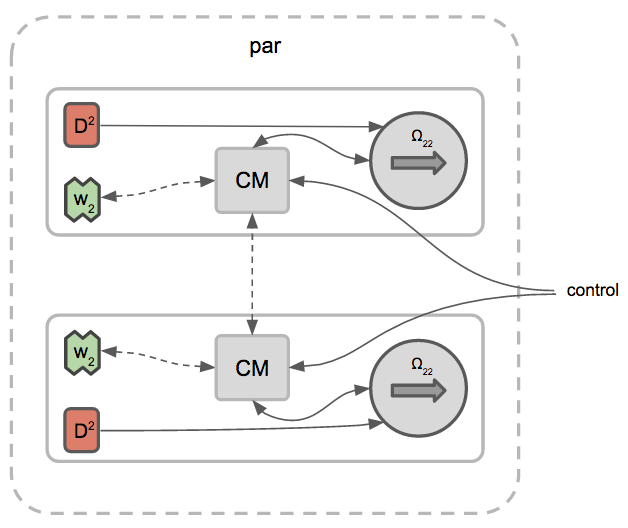
\includegraphics[width=0.5\textwidth]{img/computation_centric_consist.png}
\caption{Computation-Centric Consistency Management}
\label{fig:computation_centric_consistency}
\end{figure}
No coupling between state and framework exists, which makes it easier for a developer to reuse existing code.
Furthermore it provides a better abstraction due to the separation of logic and data and also a unit is already a part of the control-flow, responsible for executing the computational part.
Lastly, no proxy is required, which considerable simplifies the process of adding new types of state to the framework or reuse existing implementations such as matrix libraries.
In this architecture, the consistency management is periodically invoked to communicate with the driver in order to fetch new instructions and exchange progress with parallel units.

\section{Unit-internal Control-flow}
Considering both approaches, computation-centric consistency seems the best fit for the framework.
Therefore, in order to achieve the greatest flexibility and fine grained control over the consistency during algorithm execution, the consistency management is part of the unit itself.
Figure \ref{fig:unit_internal_flow} depicts the unit internal control-flow that is executed when the unit execution is triggered.
The control-flow contains the actual computation followed by a number of steps associated with consistency management.
\begin{figure}[ht]
\centering
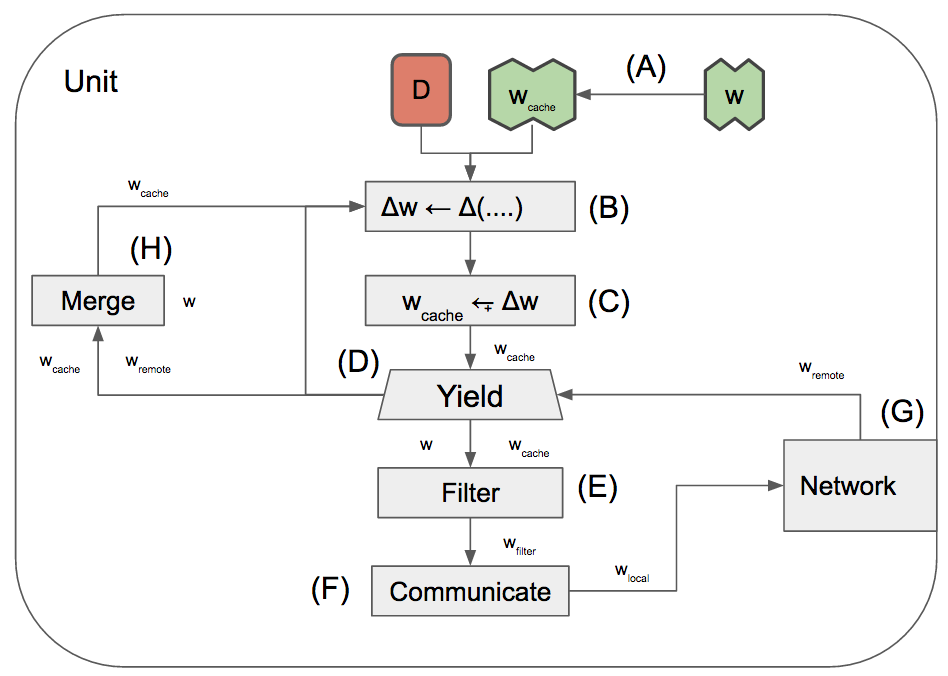
\includegraphics[width=0.9\textwidth]{img/unit_internal_flow.png}
\caption{Unit-Internal Control-flow}
\label{fig:unit_internal_flow}
\end{figure}
Previous to executing the computation enclosed in a unit, a cache is created for each state that is altered by said computation (A).
The reasoning behind this strategy is the fact that updates to the state are best communicated as relative change compared to a previous state (e.g. previous iteration), whereas the actual algorithm requires the absolute change.
In order to be able to compute a delta between two defined states, only the cache is altered and compared with the previous version before communicating updates.
After this initialization step the actual computation $\Delta(\ldots)$ is executed according to (\ref{eqn:delta_upd}), which results in a delta $\Delta w$ that can be used to update the state $w$.
Instead of applying the delta to actual state $w$, it is applied to the cache $w_{cache}$ only (C).
When running iterative-convergent algorithms this procedure of updating and caching is repeated multiple times according to the algorithm definition.
In order for the consistency management to gain a fine grained control over the update communication frequency during the execution, step (D) in the control-flow is a yield component similar to the primitive used in coroutines.
As with coroutines, the yield suspends the execution of the (update) computation in favor of executing other tasks.
In case of a unit with consistency management, the yield is triggered on request of the consistency management and at a frequency that is agreed on with the other replicas of the unit.
Upon a yield, the local progress is communicated to the other units $\Omega_{ij}$ in order to ensure a consistent state.
For this to happen, the actual state $w$ and the cached version $w_{cache}$ are used to compute $\Delta w = w_{cache} - w$, which is then forwarded to the filter stage (E) if configured.
The filter stage provides the developer with the ability to control which updates are actually forwarded to the communication stage (F) based on a defined criterion.
This is necessary for example when there is a bandwidth quota for each machine/unit and only a subset of the updates can be communicated.
All updates passing the filter stage are then forwarded to the communication stage and sent to the other units over the network.
Furthermore, if remote updates $w_{remote}$ have been received over the network, these are merged into the actual state $w$ together with the locally cached updates $w_{cache}$.
A summary of merge strategies together with filter strategies is described in the following section.


\section{Strategies}
When executing an algorithm in parallel on a cluster of machines, often additional constraints are induced by the architecture.
For example, multiple independent tasks could be executed on the same machine and therefore a quota on resources like network bandwidth is enforced on a process level.
In such cases the consistency management needs additional means to identify the updates that are most important to the algorithm progress.
Filtering or prioritizing updates allows the consistency management to identify the most important updates that need to be communicated first without exceeding the network quota.

\subsection{Filter}
The simplest strategy for prioritizing updates is randomly choosing updated parameters of the state for communication until the network quota is exceeded.
Round-robin prioritization on the other hand repeatedly selects parameters following a fixed schedule.
A more data-driven approach takes the absolute magnitude of the change
\begin{equation}
\mid\Delta w\mid = \mid w - w_{cache} \mid
\label{eqn:absolute_magnitude}
\end{equation}
into account when deciding which parameters to communicate first.
Depending on the algorithm, the relative change in magnitude
\begin{equation}
\mid\frac{\Delta w}{a} \mid = \mid\frac{w - w_{cache}}{a} \mid
\label{eqn:relative_magnitude}
\end{equation}
might be a better prioritization strategy, where $a$ is the current value of the parameter.

\subsection{Merge}
In addition to prioritization, the merging strategy must be specified as well.
Merging refers to the process of combining local updates $w_{local}$, remote updates $w_{remote}$ and the current state $w$ to form an updated version of this particular state.
Merging in general can be described by
\begin{equation}
w_{i}^{t} = w_{i}^{t-1} + \gamma\sum_{k = 0}^{K}\Delta w_{k}
\label{eqn:state_merging}
\end{equation}
where $w_i^t$ is the updated state at time $t$, computed by updating the previous version of the state with a weighted sum of the remote states updates $\Delta w_k, k \neq i$ and the local updates $\Delta w_k, k = i$.
Depending on the partitioning of the state and the algorithm employed, the parameter $\gamma$ is commonly chosen to be either $\frac{1}{K}$ (averaging) or $1$ (adding).
